% This is a sample LaTeX input file.  (Version of 9 April 1986) 
% 
% A '%' character causes TeX to ignore all remaining text on the line, 
% and is used for comments like this one.

\documentclass{article}    % Specifies the document style.
\usepackage{graphicx}
\usepackage{alltt}
\title{Ontology Engineering \& Semantic Web \\ Project Report}  % Declares the document's title. 
\author{Panagiotis Chatzichristodoulou and Kirill Tumanov}    % Declares the author's name
\date{March 27, 2014}   % Deleting this command produces today's date.

%
\begin{document}           % End of preamble and beginning of text.
%
\maketitle                 % Produces the title.
%
\begin{abstract}
%
This work serves as a reference and a summary document for the designed Student Lifecycle Management (SLM) system ontology, based on the SAP AG framework. It gives an overall structure of the ontology and describes the main functions of student lifecycle it reflects. For better comprehension this description is coupled with following the built-it exemplar individuals. The paper ends with discussion on ontology limitations and possible future work.
%
\end{abstract}
%
% 
\section{Introduction}
%
Ontology engineering is a field that studies the methods and methodologies of building ontologies. From an Artificial Intelligence point of view, an ontology is defined as: ``explicit specification of conceptualization''~\cite{Gruber}, meaning that ontologies are formal representations of sets of concepts and the relations between them within a domain. It must be noted that even though ontologies are build to serve as formal representations of a certain problem, ontologies should be build as problem-independent as possible. Consequently, an ontology about a car of a certain brand must also be able to represent cars of other brads without any modifications. The domain of the ontology described in this paper is the domain of SLM, meaning that the ontology build creates a framework that describes the SLM system. Despite the fact that it was based on SAP-SLM~\cite{sap}, the ontology can represent a much wider range of student lifecycle management systems.
% 
\section{Implementation}
%
The ontology of SLM system was designed according to the available SAP AG framework, shown in Fig.~\ref{SAP}. The implementation itself was done in Protege 4.3.0 software in the Web Ontology Language (OWL) format. HermiT 1.3.8 was used as a means of reasoning. 
\begin{figure}[htbp]
  \centering
    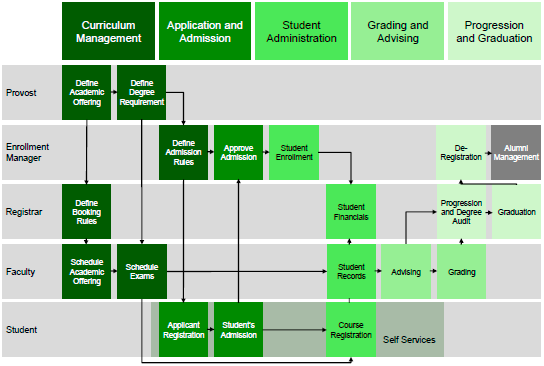
\includegraphics[width=0.8\textwidth]{Materials/Figures/1.png}
    \caption{SAP AG framework of SLM~\cite{sap}}
  \label{SAP}
\end{figure}

Although there is no clear specification of what procedures the system is able to reflect, it is relatively easy to understand what are the most essential ones. Some of the blocks shown here in the ontology were logically merged or united by their roles and underlying processes. E.g. ``Graduation" was merged with ``De-Registration" and has a lot in common with ``Define Degree Requirement". 

A more specific review of the ontology is done in the following subsections. They are organized on the built-in individuals, as a whole student lifecycle process.
%
\subsection{Application and Graduation}
%
Everything started when a British school graduate Bob Smith heard from his friend Joey Miller about the RWTH University, who graduated on the same year. Joey told him that some years ago he was a student at the Mathematics Department of this university. He followed a Study Programme in Mathematics very similar to the one in existence. Upon completion of the studies, he was awarded a BSc Degree in Mathematics, de-registered by Sam Jones - an Enrollment Manager and included into the list of RWTH Alumni. Now Joey was going to attend an Alumni Meeting organized by Terry Mitchel - an Alumni Manager.

Joey inspired Bob to take the same study programme as his, since Bob was quite into Math. So, Bob filed an Admission Request, which includes all needed documents and side procedures, this request was received and fulfilled (processed) by the Enrollment Manager. After the decision was made, the Admission Request resulted in Admission Response, which was sent to Bob. Bob received the Response and found himself accepted to the RWTH. He later was enrolled as a student by the Enrollment Manager. 
% 
\subsection{Study Programme}
%
Bob being a Math student selected to pursue a Study Programme in Mathematics, which culminates with an award of BSc Degree to the graduates. The Study Programme defined by Lilian Marshall - a Provost, apart from the rest includes Courses in Linear Algebra and Statistical Theory. The Programme and all its Courses are taught in English. In addition, the Study Programme has a number of Specializations, among which are a Major in Mathematics and a Minor in Statistics.

Graduation Requirements for each Study Programme are defined by the Provost. These requirements mainly include the number of Credits a Student must obtain for the Courses he/she completes successfully.

A certain amount of Credits is given for each Course, while it also is awarded to a Student upon a successful completion. A Course in Statistical Theory has a Linear Algebra as a prerequisite. Each Course is taught by a Faculty. Course is comprised of Lectures.

Each Lecture being an Event has its location, start and end time, which are scheduled by Kyle Nillson - a Scheduling Officer. A Person registered for the Course the Lecture is of may attend it. Each Lecture may have a different teaching method: a lecture, a practical or a seminar.

A Course may have one of the following statuses: booking, ended, fully booked or ongoing. When Course is in a booking state, a Student is able to, first, book a place in it and later to be registered. An end of a booking term is defined by the Course's booking deadline. Finally, after taking a Course a student may fail it or complete successfully.

Successful completion or failure of a Course is based on the Student's Grade obtained at the corresponding Exam. Exam is an event, like a Lecture, and thus has similar features. In addition, an Exam Paper is issued for each Exam, meaning a set of questions a Student is to answer. A Faculty member conducts an Exam, grades the Exam Paper and reports a Grade to the Student.

Bob's Linear Algebra course is taught by Jeffry Hunt - a Full Professor of Mathematics, and a Statistical Theory course by Samantha Kole - a Senior Lecturer. He is registered for both of them, and attends the first and second lectures of each one respectfully.
% 
\subsection{Student Administration}
%
A Student being enrolled at a University is obliged to pay Tuition. This part of student finances a University is concerned about. So since Bob got enrolled he was a subject of tuition payment check. 

The check is a part of the Tuition Management service of the University. In RWTH Student Administration office provides this Service, with Frank de Boer - a Registrar being responsible for it. However, as Bob just got accepted the first check was performed by the Enrollment Manager, who filed the tuition fees request and sent it to Jessica Vervier - a University Accountant. She checked the RWTH public account to see that the tuition fees were paid, thus fulfilling a request, which resulted in a positive response sent back to the Enrollment Manager.

However not only finances but all the personal information and grades of a Student are in the competence of the Student Administration office. This data is stored and retrieved from the RWTH grade and personal info databases, accessible through a University Portal in the Web. RWTH Students and personnel have different privileges using the Portal.
% 
\subsection{Advising}
%
Once Bob became a Student he started to take care of his upcoming Internship. As he was new to the procedures he decided to ask an advise of the Mathematics Department Study Advisor - Gonny Willems. To do so, Bob filed a request of additional info on the internship possibilities, which was a general e-mail on practice. Gonny received his e-mail, thought of an answer and replied, providing him a general information an useful links. Therefore, she fulfilled a request and produced a response to it.

Once Bob received this information from the Study Advisor, he contacted a company named Diamond LLC. There he was said that they had a placement - an Internship in Data Analysis. After thinking of his career prospects Bob decided to accept the offer and fill the position. Since then, in addition to being a Mathematics Student Bob also plays a Role of a Data Analyst.
% 
\subsection{Visualization}
%
This section provides and analyses visualizations of the ontology. The visualizations provided are in the form of Cloud Views. Such views provide insight about the relations between its Terminology and Application. Firstly, in Figure~\ref{classUsage} classes that are used the most in the ontology are displayed. That is the ones that have the most relations and provide the basis in which the ontology is build. As expected, the classes of \textit{Course}, \textit{StudyProgramme}, \textit{Student} and \textit{Role} play a major role in the ontology and serve as its backbone. On the other hand, classes like \textit{Database} and \textit{Document} are used much less even though they are essential to the structure of this ontology.

Secondly, information about the amount of functionality each individual within the ontology has, is displayed in Figure~\ref{cloudIndi}. Again, instances of type \textit{Course}, \textit{Role}, \textit{StudyProgramme} and \textit{Student} are the most used ones. Furthermore instances like \textit{UniversityAccountant} have much less connections despite being essential to the ontology. That is expected since some individuals provide the core of the ontology and are used more than others. That displays a good correlation between the Terminology of the ontology and its Application.
\begin{figure}[htbp]
  \centering
    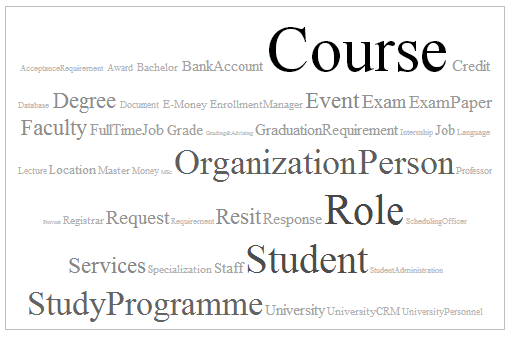
\includegraphics[width=0.8\textwidth]{Materials/Figures/classUsageCloud.png}
    \caption{Cloud view of the ontology visualizing class usage}
  \label{classUsage}
\end{figure}

\begin{figure}[htbp]
  \centering
    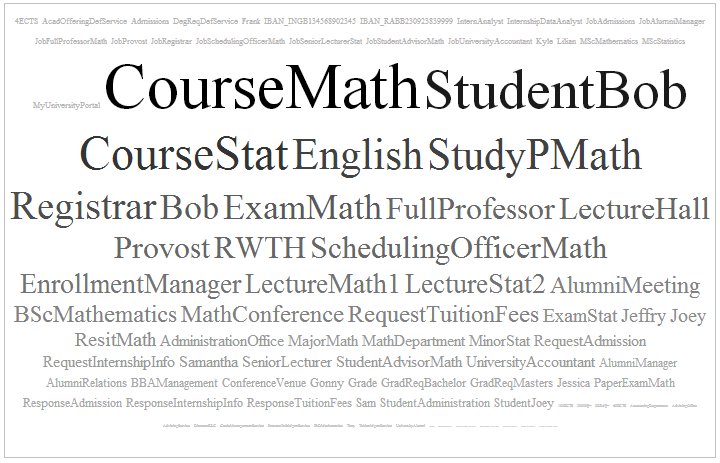
\includegraphics[width=0.8\textwidth]{Materials/Figures/cloudIndies.png}
    \caption{Cloud view of the ontology visualizing individual usage}
  \label{cloudIndi}
\end{figure}

% 
\subsection{Conclusion}
%
Building an ontology that successfully represents a problem domain is not a trivial task. It requires a correct abstraction of the notions included, and iterative restructuring of the ontology so that it has an correct structure. In this work the designed ontology's capabilities were demonstrated from the application point of view rather than the terminological one. This approach was chosen because it makes the tasks of reporting and describing the usage of the ontology easier and more complete; easier because it removes from the reader the cognition load of finding usage for the ontology, and more complete because it provides an Application to the ontology and, as a result, completes the basic Knowledge Base of it.

%
% ---- Bibliography ----
%
\begin{thebibliography}{99}
%
\bibitem {sap}
Solution in Detail: Higher Education and Research. Student Life Management.
SAP AG, \texttt{http://www.sap.com/bin/sapcom/en\_us/downloadasset.2013-12-dec\newline-11-11.higher-education-and-research-student-lifecycle-\newline management-pdf.html}(2013)

\bibitem{protege}
Protege ontology creation tool Website.\\
\texttt{http://protege.stanford.edu/}

\bibitem{protegeWiki}
Protege ontology creation tool Wiki.\\
\texttt{http://protegewiki.stanford.edu/wiki/Main\_Page}

\bibitem{protegeCloudViews}
Protege tool cloud views plugin.\\
\texttt{http://protegewiki.stanford.edu/wiki/Cloud\_Views}

\bibitem{protegeOntoGraph}
Protege onto graph views plugin.\\
\texttt{http://protegewiki.stanford.edu/wiki/OntoGraf}

\bibitem{ontoCleanPaper}
Ontoclean Method.\\
\texttt{http://www.researchgate.net/publication/27293101\_Evalu-\newline
ating\_ontological\_decisions\_with\_OntoClean/file/9fcfd50-\newline
f9621161392.pdf}

\bibitem{Gruber}
Gruber T.:
\\
\texttt{http://www-ksl.stanford.edu/kst/ what-is-an-ontology.html.} 



%%%%%%%%%%%%%%%%%%%%%%%%%%%%%%%%%%%%%%%%%%%%%%%%%%%%%%%%%%%%%%%%%%%
\end{thebibliography}
\end{document}             % End of document. 